% Template KLTN cho SV trường ĐHKHTN
% Liên hệ: nqminh@fit.hcmus.edu.vn
% Last update: 08/06/2016

% Chú ý: đọc các phần chú ý đóng khung của file này và chỉnh lại cho phù hợp.
% Trước khi build, xóa hết các file được tạo ra trong quá trình build trước đó, và build theo thứ tự: BIB > PDF > PDF.
% Nếu cập nhật tài liệu tham khảo, cũng cần build lại theo cách trên.

\documentclass[oneside,a4paper,14pt]{extreport}

% Font tiếng Việt
\usepackage[T5]{fontenc}
\usepackage[utf8]{inputenc}
\DeclareTextSymbolDefault{\DH}{T1}

% Tài liệu tham khảo
\usepackage[
	sorting=nty,
	backend=bibtex,
	defernumbers=true]{biblatex}
\usepackage[unicode]{hyperref} % Bookmark tiếng Việt
\addbibresource{References/references.bib}

\makeatletter
\def\blx@maxline{77}
\makeatother

% Chèn hình, các hình trong luận văn được để trong thư mục Images/
\usepackage{graphicx}
\graphicspath{ {Images/} }

% Chèn và định dạng mã nguồn
\usepackage{listings}
\usepackage{color}
\definecolor{codegreen}{rgb}{0,0.6,0}
\definecolor{codegray}{rgb}{0.5,0.5,0.5}
\definecolor{codepurple}{rgb}{0.58,0,0.82}
\definecolor{backcolour}{rgb}{0.95,0.95,0.92}
\lstdefinestyle{mystyle}{
    backgroundcolor=\color{backcolour},   
    commentstyle=\color{codegreen},
    keywordstyle=\color{magenta},
    numberstyle=\tiny\color{codegray},
    stringstyle=\color{codepurple},
    basicstyle=\footnotesize,
    breakatwhitespace=false,         
    breaklines=true,                 
    captionpos=b,                    
    keepspaces=true,                 
    numbers=left,                    
    numbersep=5pt,                  
    showspaces=false,                
    showstringspaces=false,
    showtabs=false,                  
    tabsize=2
}
\lstset{style=mystyle}

% Chèn và định dạng mã giả
\usepackage{amsmath}
\usepackage{algorithm}
\usepackage[noend]{algpseudocode}
\makeatletter
\def\BState{\State\hskip-\ALG@thistlm}
\makeatother

% Bảng biểu
\usepackage{multirow}
\usepackage{array}
\newcolumntype{L}[1]{>{\raggedright\let\newline\\\arraybackslash\hspace{0pt}}m{#1}}
\newcolumntype{C}[1]{>{\centering\let\newline\\\arraybackslash\hspace{0pt}}m{#1}}
\newcolumntype{R}[1]{>{\raggedleft\let\newline\\\arraybackslash\hspace{0pt}}m{#1}}

% Đổi tên mặc định
\renewcommand{\chaptername}{Chương}
\renewcommand{\figurename}{Hình}
\renewcommand{\tablename}{Bảng}
\renewcommand{\contentsname}{Mục lục}
\renewcommand{\listfigurename}{Danh sách hình}
\renewcommand{\listtablename}{Danh sách bảng}
\renewcommand{\appendixname}{Phụ lục}

% Dãn dòng 1.5
\usepackage{setspace}
\onehalfspacing

% Thụt vào đầu dòng
\usepackage{indentfirst}

% Canh lề
\usepackage[
  top=30mm,
  bottom=25mm,
  left=30mm,
  right=20mm,
  includefoot]{geometry}
  
% Trang bìa
\usepackage{tikz}
\usetikzlibrary{calc}
\newcommand\HRule{\rule{\textwidth}{1pt}}

% ========================================================================================= %
% CHÚ Ý: Thông tin chung về KLTN - sinh viên điền vào đây để tự động update các trang khác  %
% ========================================================================================= %
\newcommand{\tenSV}{Nguyễn~Văn~A~-~Trần~Văn~B} % Dấu ~ là khoảng trắng không được tách (các chữ nối với nhau bằng dấu ~ sẽ nằm cùng 1 dòng
\newcommand{\mssv}{1234567}
\newcommand{\tenKL}{Sử~dụng~LaTeX trong Khoá~luận~tốt~nghiệp} % Chú ý dấu ~ trong tên khóa luận
\newcommand{\tenGVHD}{Tên~Giáo~Viên}
\newcommand{\tenBM}{Công nghệ tri thức}

\begin{document}

\begin{titlepage}

\begin{center}
%ĐẠI HỌC QUỐC GIA THÀNH PHỐ HỒ CHÍ MINH\\
TRƯỜNG ĐẠI HỌC KHOA HỌC TỰ NHIÊN\\
\textbf{KHOA CÔNG NGHỆ THÔNG TIN}\\[2cm]


{ \Large \bfseries Bùi Huy Thông\\[2cm] } 

%Tên đề tài Khóa luận tốt nghiệp/Đồ án tốt nghiệp

{ \Large \bfseries QUẢN LÝ VÀ CHIA SẺ NỘI DUNG SỐ \\ PHI TẬP TRUNG \\[3cm]} 


%Chọn trong các dòng sau
\large LUẬN VĂN THẠC SĨ KHOA HỌC MÁY TÍNH\\
%\large ĐỒ ÁN TỐT NGHIỆP CỬ NHÂN\\
%\large THỰC TẬP TỐT NGHIỆP CỬ NHÂN\\
%Đưa vào dòng này nếu thuộc chương trình Chất lượng cao, hoặc lớp Cử nhân tài năng
%\large CHƯƠNG TRÌNH CHÍNH QUY\\
%\large CHƯƠNG TRÌNH CHẤT LƯỢNG CAO\\
%\large CHƯƠNG TRÌNH CỬ NHÂN TÀI NĂNG\\[2cm]


\begin{tikzpicture}[remember picture, overlay]
  \draw[line width = 2pt] ($(current page.north west) + (2cm,-2cm)$) rectangle ($(current page.south east) + (-1.5cm,2cm)$);
\end{tikzpicture}

\vfill
Tp. Hồ Chí Minh, tháng MM/YYYY

\end{center}

\pagebreak



\begin{center}

TRƯỜNG ĐẠI HỌC KHOA HỌC TỰ NHIÊN\\
\textbf{KHOA CÔNG NGHỆ THÔNG TIN}\\[2cm]


{\large \bfseries Bùi Huy Thông - 2611030\\} 


%Tên đề tài Khóa luận tốt nghiệp/Đồ án tốt nghiệp

{ \Large \bfseries QUẢN LÝ VÀ CHIA SẺ NỘI DUNG SỐ \\ PHI TẬP TRUNG \\[2cm]}  


%Chọn trong các dòng sau
\large LUẬN VĂN THẠC SĨ KHOA HỌC MÁY TÍNH\\
%\large ĐỒ ÁN TỐT NGHIỆP CỬ NHÂN\\
%Đưa vào dòng này nếu thuộc chương trình Chất lượng cao, hoặc lớp Cử nhân tài năng
%\large CHƯƠNG TRÌNH CHÍNH QUY\\[2cm]
%\large CHƯƠNG TRÌNH CHẤT LƯỢNG CAO\\[2cm]
%\large CHƯƠNG TRÌNH CỬ NHÂN TÀI NĂNG\\[2cm]

\textbf{NGƯỜI HƯỚNG DẪN}\\
PGS.TS. Nguyễn Đình Thúc\\


\begin{tikzpicture}[remember picture, overlay]
  \draw[line width = 2pt] ($(current page.north west) + (2cm,-2cm)$) rectangle ($(current page.south east) + (-1.5cm,2cm)$);
\end{tikzpicture}

\vfill
Tp. Hồ Chí Minh, tháng MM/YYYY

\end{center}

\end{titlepage}
% Sasu trang Title, các bạn chèn nhận xét gủa GVHD và GVPB. Nhận xét sẽ được giáo vụ phát sau buổi bảo vệ để các bạn đóng quyển.

\pagenumbering{roman} % Đánh số i, ii, iii, ...

%\addcontentsline{toc}{chapter}{Lời cam đoan}
%\chapter*{Lời cam đoan}
\label{reassurances}

Tôi xin cam đoan đây là công trình nghiên cứu của riêng tôi. Các số liệu và kết quả nghiên cứu trong luận văn này là trung thực và không trùng lặp với các đề tài khác.

\addcontentsline{toc}{chapter}{Lời cảm ơn}
\chapter*{Lời cảm ơn}

Tôi xin chân thành cảm ơn ...

\addcontentsline{toc}{chapter}{Đề cương chi tiết}
\include{Appendix/decuong}

% Mục lục, danh sách hình, danh sách bảng
\addcontentsline{toc}{chapter}{Mục lục}
\tableofcontents
\listoffigures
\listoftables

\addcontentsline{toc}{chapter}{Tóm tắt}
\include{Appendix/tomtat}

\clearpage

\pagenumbering{arabic} % Đánh số 1, 2, 3, ...

% Các chương nội dung
\chapter{Giới thiệu}
\label{Chapter1}

%Tóm tắt luận văn được trình bày nhiều nhất trong 24 trang in trên hai mặt giấy, cỡ chữ Times New Roman 11 của hệ soạn thảo Winword hoặc phần mềm soạn thảo Latex đối với các chuyên ngành thuộc ngành Toán.

%Mật độ chữ bình thường, không được nén hoặc kéo dãn khoảng cách giữa các chữ.
%Chế độ dãn dòng là Exactly 17pt.
%Lề trên, lề dưới, lề trái, lề phải đều là 1.5 cm.
%Các bảng biểu trình bày theo chiều ngang khổ giấy thì đầu bảng là lề trái của trang.
%Tóm tắt luận án phải phản ảnh trung thực kết cấu, bố cục và nội dung của luận án, phải ghi đầy đủ toàn văn kết luận của luận án.
%Mẫu trình bày trang bìa của tóm tắt luận văn (phụ lục 1).

\noindent \textit{Trong chương này, đầu tiên nhóm chúng em phát biểu về bài toán đề xuất sản phẩm cũng như là ý nghĩa của nó đối với cuộc sống hiện nay. Sau đó, nhóm chúng em trình bày về vấn đề thiên lệch dữ liệu, một thách thức lớn của bài toán đề xuất sản phẩm. Từ đó dẫn đến phương pháp nhóm chúng em tìm hiểu ``Inverse propensity scoring'' (IPS) để khắc phục vấn đề thiên lệch dữ liệu này. Ngoài ra, ở cuối chương nhóm chúng em sẽ trình bày về cách tổ chức của khóa luận.}

\section{Phát biểu và ý nghĩa của bài toán}
Ngày nay, các loại sản phẩm phục vụ cho đời sống con người được sinh ra ngày một nhiều. Điều này tạo nên thách thức cho người dùng là làm thế nào để có thể tìm thấy được các sản phẩm phù hợp với bản phân giữa một lượng sản phẩm khổng lồ như vậy. Do đó hệ thống đề xuất sản phẩm đã ra đời nhằm mục đích hỗ trợ cho người dùng trong quá trình tìm kiếm nội dung phù hợp cho bản thân..

Các hệ thống đề xuất sản phẩm giúp cho trải nghiệm của người dùng được cá nhân hóa, giúp tiết kiệm thời gian cho người dùng trong việc lựa chọn sản phẩm. Mặt khác, đối với các công ty nó còn tăng cao lợi thế cạnh tranh, kích thích nhu cầu mua sắm của người dùng bằng các gợi ý sản phẩm. Có thể kể đến các hệ thống đề xuất sản phẩm nổi tiếng như: hệ thống đề xuất phim của Netflix, hay hệ thống đề xuất video của Youtube, hệ thống đề xuất nhạc của Spotify và nhiều loại hệ thống đề xuất khác nữa.

Bài toán hệ thống đề xuất sản phẩm sẽ được phát biểu như sau (hình \ref{fig:chap1_rs} minh hoạ về cách thức hoạt động của hệ thống đề xuất phim):
\begin{itemize}
    \item Đầu vào là dữ liệu về điểm đánh giá của các người dùng đối với các sản phẩm trong hệ thống; dữ liệu này sẽ được đưa vào mô hình dưới dạng một ma trận tương tác thưa với mỗi dòng là các đánh giá của người dùng cho các sản phẩm. Ngoài ra, còn có thể có thêm dữ liệu về thông tin của mỗi người dùng và mỗi sản phẩm; dữ liệu này được đưa vào mô hình dưới dạng 2 ma trận thuộc tính của người dùng và sản phẩm, các điểm dữ liệu trong ma trận thuộc tính sẽ được tiền xử lý thành dạng số.

    \item Yêu cầu: đề xuất các sản phẩm trong hệ thống mà phù hợp với sở thích của mỗi người dùng (để có thể đề xuất thì một cách làm phổ biến là dự đoán điểm đánh giá của người dùng đối với các sản phẩm mà người dùng chưa đánh giá).
\end{itemize}

\begin{figure}[h]
    \centering
    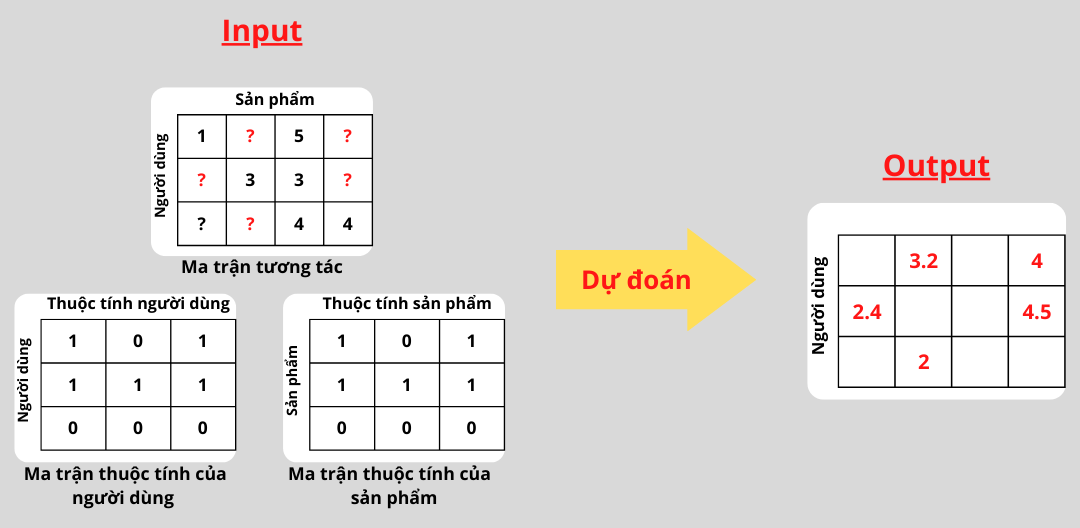
\includegraphics[width=\textwidth]{images/Chapter1/rs.png}
    \caption{Cách thức hoạt động của hệ thống đề xuất sản phẩm}
    \label{fig:chap1_rs}
\end{figure}

Cụ thể hơn, đầu vào của hệ thống sẽ là ma trận tương tác (chứa điểm đánh giá của các người dùng cho

Trong phạm vi đề tài của khóa luận nhóm chúng em sẽ tiến hành xử lý trên dữ liệu explicit feedback. Explicit feedback là dữ liệu cho biết rõ ràng mức độ ưa thích của người dùng đối với sản phẩm, chẳng hạn như điểm đánh giá của người dùng cho 1 bộ phim từ 1 đến 5. 


\section{Thách thức của bài toán}
\label{section:thachthuc}
Để huấn luyện được mô hình có thể đề xuất chính xác tất cả các sản phẩm cho người dùng, ta cần một bộ dữ liệu đầy đủ bao gồm đánh giá của tất cả người dùng cho tất cả sản phẩm. Tuy nhiên dữ liệu này không thể có được trong thực tế, do người dùng không thể nào xem và đánh giá tất cả các sản phẩm trong hệ thống. Vì vậy để mô hình có thể huấn luyện được tốt nhất ta cần bộ dữ liệu quan sát được phải được phát sinh từ phân phối đều của bộ dữ liệu đầy đủ này, vì bộ dữ liệu quan sát được này sẽ đại diện cho bộ dữ liệu đầy đủ và nó được gọi là dữ liệu không bị thiên lệch. 

Dữ liệu quan sát được trong bài toán đề xuất sản phẩm thường bị gặp vấn đề lớn về thiên lệch dữ liệu. Thiên lệch dữ liệu là dữ liệu quan sát được không được phát sinh từ phân phối đều, do đó nó không đại diện được cho bộ dữ liệu đầy đủ. Bắt nguồn từ 2 nguyên nhân chính trong việc thu thập dữ liệu sau:
\begin{itemize}
    \item Do người dùng tự chọn các bộ phim để đánh giá, thay vì dựa trên việc người dùng đánh giá một tập các sản phẩm ngẫu nhiên.
    Việc người dùng đánh giá trên một tập các sản phẩm được đề xuất ngẫu nhiên sẽ đảm bảo dữ liệu thu được được phát sinh từ phân phối đều, giúp cho dữ liệu thu được có thể đại diện được cho tập dữ liệu đầy đủ.
    Một kết quả nghiên cứu của tác giả Marlin và các cộng sự \cite{bias} đã cho thấy tác động rõ ràng của thiên lệch dữ liệu. Họ đã tiến hành một cuộc khảo sát người dùng để thu thập dữ liệu điểm đánh giá của người dùng đối với một số sản phẩm được lựa chọn ngẫu nhiên, để so sánh với các sản phẩm do người dùng tự lựa chọn. Hình \ref{fig:self_selection_bias} cho thấy rõ sự khác nhau trong phân phối dữ liệu của việc lựa chọn ngẫu nhiên và do người dùng đánh giá và đưa ra 2 phát hiện: 1) người dùng có xu hướng chọn và đánh giá các mặt hàng họ thích; và 2) người dùng có nhiều khả năng xếp hạng các mặt hàng đặc biệt xấu hoặc đặc biệt tốt.
    \item Do hệ thống đề xuất chỉ chọn các bộ phim nào đó để hiển thị cho người dùng, trong trường hợp hệ thống đề xuất sản phẩm đã triển khai từ trước. Với tác động của hệ thống đề xuất như vậy, người dùng chỉ có thể xem và đánh giá trên các bộ phim được hiển thị, điều này làm cho dữ liệu thu thập được chỉ tập trung vào một vài loại sản phẩm nào đó, không đại diện cho toàn bộ dữ liệu.
\end{itemize}

\begin{figure}
    \centering
    \begin{subfigure}[b]{0.4\textwidth}
     \centering
     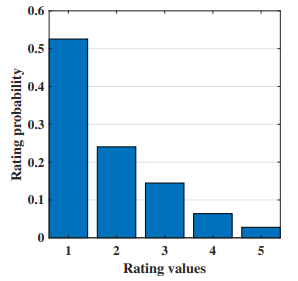
\includegraphics[width=\textwidth]{images/Chapter1/bias_1.png}
     \caption{Các sản phẩm được chọn ngẫu nhiên.}
     \label{fig:randomly_selected}
    \end{subfigure}
    \hfill
    \begin{subfigure}[b]{0.4\textwidth}
     \centering
     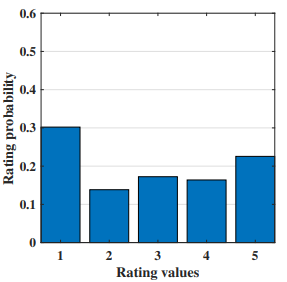
\includegraphics[width=\textwidth]{images/Chapter1/bias_2.png}
     \caption{Các sản phẩm được chọn do người dùng tự lựa chọ.n}
     \label{fig:user_selected}
    \end{subfigure}
    \caption{Phân phối điểm đánh giá sản phẩm, được thu thập bằng cách cho người dùng đánh giá các sản phẩm ngẫu nhiên và cho người dùng đánh giá các sản phẩm tự lựa chọn.}
    \label{fig:self_selection_bias}
\end{figure}

Để hiểu rõ hơn về vấn đề thiên lệch dữ liệu ta sẽ xem xét một ví dụ nhỏ trong hệ thống đề xuất phim, minh họa tác động của thiên lệch dữ liệu có thể gây ra cho việc đánh giá mô hình. Hình \ref{fig:chap1_ex_1} minh họa cho thí nghiệm của ta trong đó:
\begin{itemize}
    \item Ma trận $Y$ là ma trận đầy đủ chứa đánh giá của tất cả người dùng đối với tất cả các sản phẩm, trong ma trận này bao gồm 2 nhóm nhỏ: 1) những người dùng yêu thích phim kinh dị, họ sẽ đánh giá 5 điểm cho tất cả các phim kinh dị và 1 điểm cho tất cả các phim lãng mãn mà họ đã xem; nhóm trái ngược 2) những người dùng yêu thích phim lãng mạn, họ sẽ đánh giá 1 điểm cho tất cả các phim kinh dị và 5 điểm cho tất cả các phim lãng mạn mà họ đã xem; và cả 2 nhóm người dùng đều đánh giá cho  thể loại phim kịch là 3. 
    \item Ma trận $O$ là ma trận nhị phân chứa 2 giá trị 0 và 1, đại diện cho những sản phẩm người dùng đã đánh giá trong hệ thống, \( [O_{u,i}~=~1]\Leftrightarrow[Y_{u,i} \) được quan sát].
\end{itemize}

\begin{figure}[h]
    \centering
    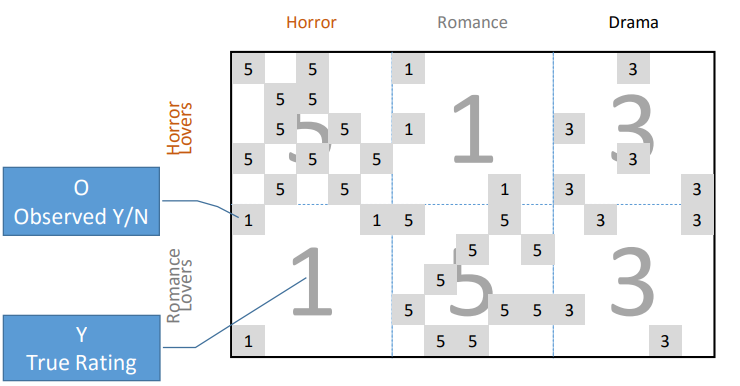
\includegraphics[width=\textwidth]{images/Chapter1/example_bias_1.png}
    \caption{Ví dụ minh họa tác động của thiên lệch dữ liệu. 
    $Y$ là những điểm đánh giá thật của dữ liệu, minh họa bằng những con số nằm bên dưới ma trận.
    $O$ là những điểm đánh giá quan sát được, minh họa bằng những điểm đánh giá của người dùng cho các sản phẩm.}
    \label{fig:chap1_ex_1}
\end{figure}

Xét 2 cách dự đoán $\hat{Y}_1$ và  $\hat{Y}_2$ sẽ được dùng để dự đoán giá trị cho các điểm đánh giá chưa quan sát được. Hình \ref{fig:chap1_ex_2} sẽ minh họa cách 2 mô hình dự đoán như sau:
\begin{itemize}
    \item Ở cách dự đoán $\hat{Y}_1$, những điểm đánh giá có giá trị thật là 1 sẽ được dự đoán là 5, các điểm đánh giá có giá trị thật là 3 và 5 sẽ được dự đoán đúng giá trị.
    \item Ở cách dự đoán $\hat{Y}_2$, những điểm đánh giá có giá trị thật là 3 sẽ được dự đoán là 5, các điểm đánh giá có giá trị thật là 3 và 5 sẽ được dự đoán đúng giá trị.
\end{itemize}

\begin{figure}[h]
    \centering
    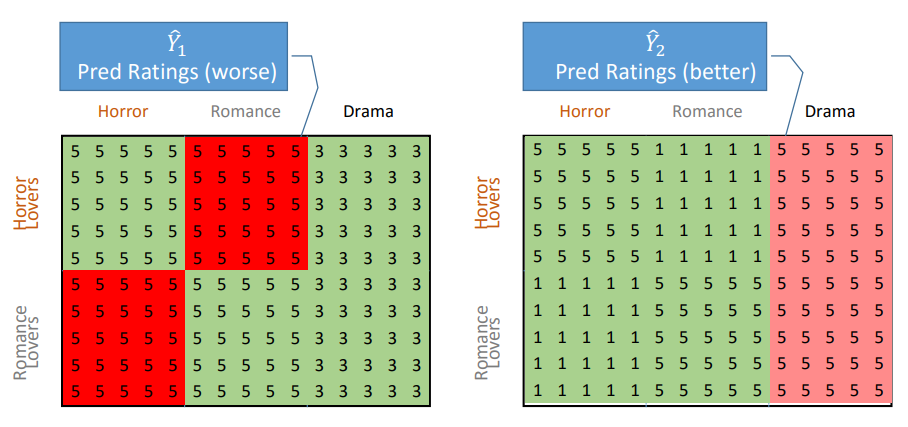
\includegraphics[width=\textwidth]{images/Chapter1/example_bias_2.png}
    \caption{Các cách dự đoán $\hat{Y}_1$ và $\hat{Y}_2$ trên tập dữ liệu}
    \label{fig:chap1_ex_2}
\end{figure}

Nếu chúng ta có thể quan sát toàn bộ dữ liệu như trong hình \ref{fig:chap1_ex_2}, ta có thể thấy với cách dự đoán $\hat{Y}_1$ khi giá trị thật là 1 nhưng dự đoán là 5 thì độ lỗi của nó rất lớn. Khi so với cách dự đoán $\hat{Y}_2$ khi giá trị thật là 3 và dự đoán là 5 có độ lỗi không quá nghiêm trọng như cách dự đoán $\hat{Y}_1$ .

Để đánh giá một cách dự đoán có tốt hay không, ta sẽ tiến hành đánh giá độ lỗi trên tập dữ liệu quan sát được. Tuy nhiên dữ liệu quan sát được ở đây lại không được phát sinh từ phân phối đều do đó nó có sự thiên lệch, cụ thể hơn là những điểm đánh giá là 1 xuất hiện ít hơn những điểm đánh giá là 3 (minh họa ở hình \ref{fig:chap1_ex_3}); điều này bắt nguồn từ việc người dùng tự lựa chọn các bộ phim họ thích để đánh giá.

Khi đánh giá cách dự đoán nào là tốt trên tập dữ liệu quan sát được bị thiên lệch này, ta sẽ cho rằng dự đoán $\hat{Y}_1$ tốt hơn $\hat{Y}_2$. Vì theo cách dự đoán $\hat{Y}_1$ những điểm có độ lỗi lớn (điểm đánh giá thật là 1 nhưng dự đoán là 5) xuất hiện rất ít trong bộ dữ liệu quan sát được; trong khi đó theo cách dự đoán $\hat{Y}_2$ những điểm có độ lỗi nhỏ hơn (điểm đánh giá thật là 3 nhưng dự đoán là 5) xuất hiện nhiều hơn trong bộ dữ liệu quan sát được; điều này làm cho độ lỗi của cách dự đoán $\hat{Y}_1$ thấp hơn cách dự đoán $\hat{Y}_2$ mặc dù cách dự đoán $\hat{Y}_1$ tệ hơn. 

\begin{figure}[h]
    \centering
    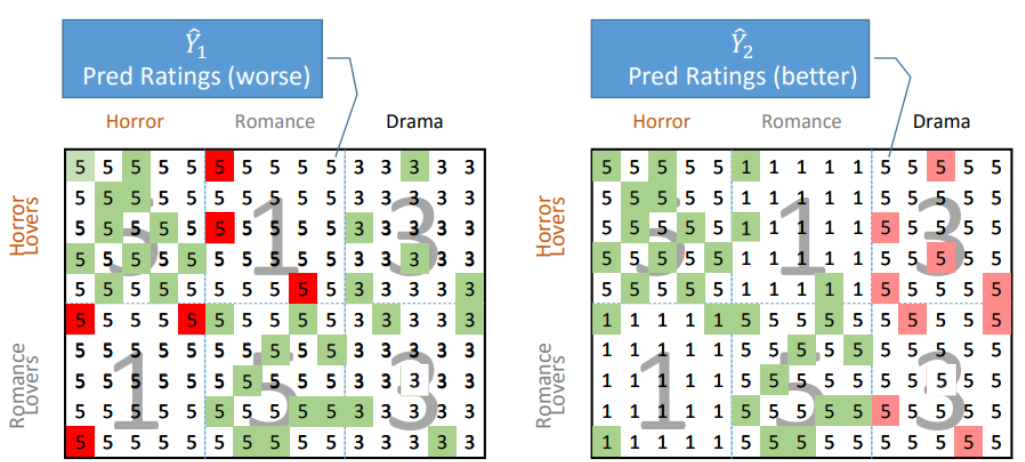
\includegraphics[width=\textwidth]{images/Chapter1/example_bias_3.png}
    \caption{Đánh giá 2 mô hình dự đoán $\hat{Y}_1$, $\hat{Y}_2$ dựa trên các mâu quan sát được }
    \label{fig:chap1_ex_3}
\end{figure}

Để khắc phục vấn đề thiên lệch dữ liệu tác giả Tobias Schnabel và các cộng sự \cite{IPS} trong bài báo ``Recommendations as Treatments: Debiasing Learning and Evaluation'' tại hội nghị ``ICML 2016'', đã đề xuất việc áp dụng phương pháp ``Inverse propensity scoring'' (IPS) vào quá trình huấn luyện và đánh giá mô hình. IPS hoạt động bằng cách đánh lại trọng số của các mẫu dựa trên điểm số xu hướng, theo cách giảm trọng số của các mẫu thường quan sát được, trong khi tăng trọng số của các mẫu hiếm gặp. Điều này sẽ giúp kiểm soát được vấn đề thiên lệch của dữ liệu.

\section{Bố cục}
Phần còn lại của khóa luận sẽ được trình bày như sau:
\begin{itemize}
    \item Chương 2 trình bày kiến thức nền tảng về ``Matrix factorization'', ``Gradient descent'', ``Naive bayes'' và ``Logistic regression''.
    \item Chương 3 trình bày về độ đo IPS và ứng dụng của nó trong việc đánh giá và huấn luyện mô hình; đây là phần chính của khóa luận. Trong phần này gồm có hai phần nhỏ:
    \begin{itemize}
        \item Độ đo ``Self normalized inverse propensity scoring'' (SNIPS). 
        \item Ước lượng ma trận xu hướng: nhóm chúng em trình bày về cách ước lượng ma trận xu hướng thông qua 2 mô hình ``Naive bayes'' và ``Logistic regression''.
    \end{itemize}
    \item Chương 4 trình bày về các thí nghiệm và các kết quả đạt được.
    \item Cuối cùng, tổng kết và các hướng phát triển sẽ được trình bày ở chương 5.
\end{itemize}


\chapter{Kiến thức nền tảng}
\label{Chapter2}

Trong chương này, đầu tiên nhóm chúng em trình bày về thuật toán ``Matrix factorization'' - thuật toán đề xuất sản phẩm bằng cách phân rã ma trận tương tác. Sau đó nhóm chúng em sẽ trình bày về thuật toán ``Gradient descent'' - thuật toán mà nhóm chúng em sẽ sử dụng để cực tiểu hóa hàm chi phí của  ``Matrix factorization''. Ngoài ra, nhóm chúng em còn trình bày về ``Naive bayes'' và ``Logistic regression'' - hai mô hình phân lớp mà nhóm chúng em sẽ sử dụng để tìm ma trận xu hướng trong IPS. Chương này, đặc biệt là về phần ``Matrix factorization'' cung cấp những kiến thức nền tảng để có thể hiểu rõ về những cải tiến mà nhóm em tìm hiểu ở chương kế tiếp.

\section{``Matrix factorization''}
``Matrix factorization'' là một phương pháp thuộc nhóm lọc cộng tác (collaborative filtering), một nhóm các phương pháp tập trung vào mối quan hệ giữa các người dùng dựa trên đánh giá của các người dùng trong hệ thống. 
Phương pháp ``Matrix factorization'' sẽ phân tích ma trận tương tác $R \in \mathbb{R}^{m \times n}$ thành tích của hai ma trận $P \in \mathbb{R}^{m \times k}$ và $\mathbf{W} \in \mathbb{R}^{k \times n}$ (hình \ref{fig:chap2_MF1} mình họa về việc phân tách ma trận tương tác $R$), trong đó: $P$ và  $Q$ là ma trận đặc trưng của người dùng và sản phẩm; $k$ là hyperparameter được điều chỉnh trong quá trình huấn luyện mô hình, đại diện cho kích thước của đặc trưng tiềm ẩn.

\begin{figure}[h]
    \centering
    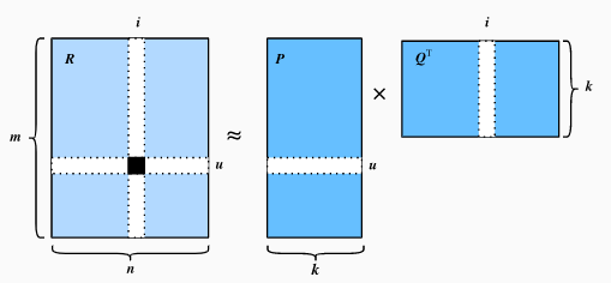
\includegraphics[width = \textwidth]{Chapter2/MF1.png}
    \caption{Matrix Factorization. Ma trận tương tác $R$ sẽ được phân rã thành ma trận đại diện cho người dùng $P$ và đại diện cho sản phẩm $Q$}
    \label{fig:chap2_MF1}
\end{figure}

Ma trận tương tác $R$ là ma trận thưa có kích thước là $m \times n$ chứa đánh giá của $m$ người dùng đối với $n$ sản phẩm có trong hệ thống. Đánh giá của người dùng $u$ cho sản phẩm $i$ trong ma trận tương tác sẽ được kí hiệu là $R_{u,i}$. Trong ma trận $P$ hàng thứ u sẽ được kí hiệu là $p_u$ và hàng thứ i trong ma trận $Q$ sẽ được kí hiệu là $q_i$.

Các đặc trưng tiềm ẩn trong $k$ mô tả sự liên quan giữa các người dùng và sản phẩm. Ví dụ như trong hệ thống đề xuất phim, các đặc trưng tiềm ẩn có thể là thể loại, ngôn ngữ, diễn viên hay bất kì các đặc trưng nào khác; hoặc có thể là bất cứ sự liên quan giữa người dùng và sản phẩm nào đó mà ta không thể giải thích được.
Mỗi sản phẩm $i$ trong ma trận sản phẩm $Q$ sẽ mang đặc trưng ẩn ở một mức độ nào đó tương ứng với các hệ số trong véc-tơ $q_i$ của nó, hệ số càng cao tương ứng với sản phẩm $i$ mang đặc trưng đó càng lớn. Tương tự, mỗi người dùng $u$ trong ma trận người dùng $P$ sẽ thích các đặc trưng ẩn này theo một mức độ nào đó tương ứng với các hệ số trong véc-tơ $p_u$, hệ số càng cao tương ứng với người dùng $u$ sẽ càng thích các bộ phim mang đặc trưng đó. Vì vậy, mục tiêu của chúng ta là sẽ đề xuất
cho người dùng $u$ những sản phẩm $i$ mang đặc trưng mà người dùng $u$ thích, tương ứng với giá trị của $p_u$ và $q_i$ đều cao dẫn đến $p_u \times q_i$ càng cao.









\section{``Gradient descent''}


\section{``Naive bayes''}


\section{``Logistic regression''}



\chapter{Phương pháp tìm hiểu}
\label{Chapter3}

Chương này nhóm chúng em trình bày về những đóng góp của bài báo mà nhóm chúng em tìm hiểu được. Ở đây, nhóm chúng em tập trung vào việc xử lý vấn đề thiên lệch dữ liệu, bằng cách sử dụng độ đo khắc phục thiên lệch IPS trong quá trình đánh giá và huấn luyện mô hình. Sau đó, nhóm chúng em trình bày về ``Self Normalized Inverse Propensity Scoring'' (SNIPS) và so sánh với IPS để thấy được sự kết nối giữa IPS và SNIPS cũng như là những điểm lợi và hại của IPS so với SNIPS. Ngoài ra, nhóm chúng em còn trình bày về phương pháp ước lượng ma trận để phục vụ cho việc tính toán độ đo IPS và SNIPS.

\section{Xem hệ thống gợi ý như một điều trị}
Như đã trình bày ở ví dụ về thiên lệch dữ liệu, ta có thể thấy rằng ta chỉ đang quan sát được một phần của dữ liệu mà không thể thấy được toàn bộ sự thật, điều này bị ảnh hưởng bởi rất nhiều yếu tố tiềm ẩn. Giống như việc khi ta muốn xem xét một loại thuốc hay một phương pháp điều trị nhất định có hiệu quả như thể nào đối với bệnh nhân,  giả sử ta tiến hành thử nghiệm phương pháp điều trị đó trên một nhóm bệnh nhân, sau đó ta theo dõi tình trạng bệnh của các bệnh nhân đó, và ta quan sát được sức khỏe của bệnh nhân có chuyển biến tích cực, liệu ta có thể kết luận được rằng phương pháp điều trị đó có thật sự hiệu quả không? Nếu xem xét kĩ lưỡng, có thể rằng phương pháp điều trị của ta có lẽ  khá đắt tiền nên chỉ những người có điều kiện kinh tế ổn định mới có xu hướng dễ tiếp xúc với phương pháp điều trị đó. Mà những người như vậy thì sẽ nhiều điều kiện thuận lợi để chăm sóc sức khỏe bản thân hơn, dẫn đến việc tình trạng bệnh của họ có chuyển biến tích cực hơn. Do đó viêc kiểm tra được độ hiệu quả một phương pháp điều trị không hề đơn giản, người ta thường sử dụng các mô hình nhân quả. Nếu ta xem mỗi người dùng như một bệnh nhân, mỗi bộ phim ta gợị ý giống như một phương pháp điều trị hoặc một loại thuốc, ta sẽ quan tâm đến việc người dùng có phù hợp với bộ phim mà ta gợi ý hay không, phim được gợi ý có khiến người dùng thích thú hay không. Từ đó ta có thể thấy bài toán gợi ý và bài toán được đưa ra khá tương đồng nhau, do có ta cũng sử dụng ý tưởng giải quyết của các phương pháp nhân quả đối với bài toán xem xét hiệu quả điều trị để gợi ý sản phẩm. 

Trong ví dụ về xem xét hiệu quả của một phương pháp điều trị, ta thấy được rằng ta cần phải kiếm soát cả những biến làm ảnh hưởng đến xu hướng mà bệnh nhân có thể tiếp cận được với điều trị đó để mô hình trở nên chính xác hơn, ví dụ như những đặc trưng về nhân khẩu học, thu nhập, mức sống, vị trí sống,... Tuy nhiên sẽ có rất nhiều biến ẩn như vậy mà ta khó có thể kiểm soát  được. Do đó phương pháp nghịch đảo điểm xu hướng ra đời (Inverse propensity scoring - IPS) với ý tưởng rằng ta không cần phải kiếm soát trực tiếp những biến ẩn, mà chỉ cần kiếm soát được xu hướng nhận được điều trị của những bệnh nhân. 

Trong bài toán gợi ý, với giả định rằng người dùng có thể đánh giá hoặc không đánh giá một phim mà họ đã xem, một đánh giá của người dùng dành cho một sản phẩm có thể xuất hiện hoặc không xuất hiện trong tập dữ liệu mà ta qua sát được. Ta có thể biểu diễn điều này thông qua ma trận quan sát O, trong đó các giá trị $O_{u,i}=1$ tương ứng với đánh giá cho bộ phim i từ người dùng u được cung cấp tới hệ thống. Ta đặt $P_{u,i}$ là xác suất mà đánh giá $Y_{u,i}$ có thể quan sát được, hay  $P_{u,i} = P(O_{u,i} = 1)$.  $P_{u,i}$ được gọi là điểm xu hướng của đánh giá  $Y_{u,i}$. Từ các đặc trưng mà ta đã quan sát được về các người dùng, các bộ phim và ma trận quan sát O, ta có thể dự đoán được điểm xu hướng của ma trận đánh giá Y. Phương pháp này sẽ được giới thiệu ở phần tiếp theo của khóa luận này.


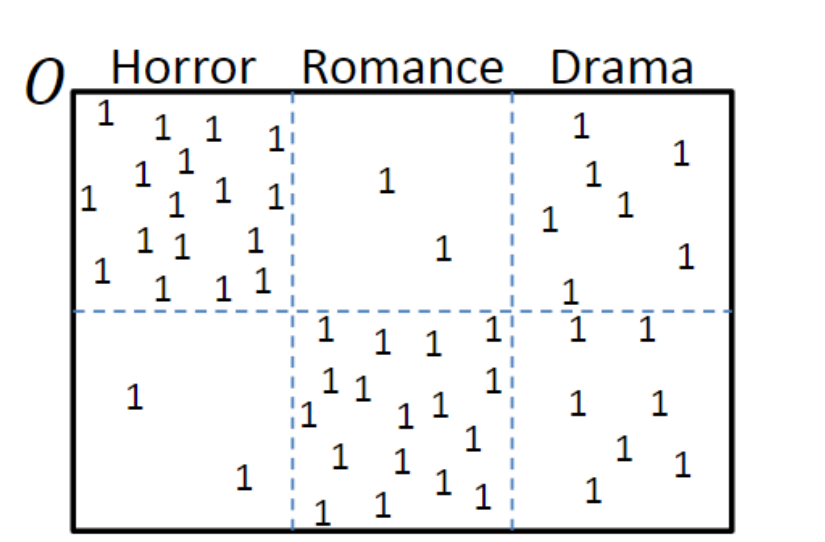
\includegraphics[width=\textwidth]{images/Chapter3/O.png}


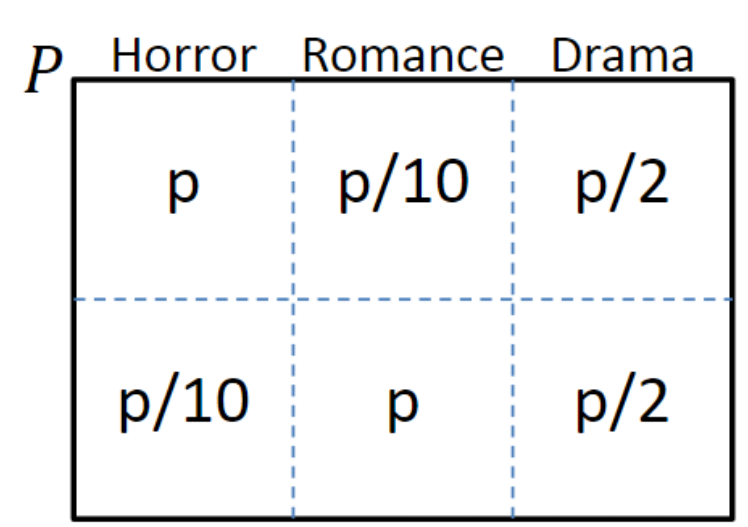
\includegraphics[width=\textwidth]{images/Chapter3/P.png}


Hình ảnh trên minh họa về việc biểu diễn ma trận quan sát O và ma trận xu hướng P. Trong ma trận quan sát O các vị trí có giá trị là 1 đại diện cho đánh giá của người dùng với sản phẩm xuất hiện trong hệ thống, ma trận xu hướng P chứa xu hướng của các đánh giá tương ứng với khả năng ta quan sát được các đánh giá, những phim có số lượt đánh giá nhiều sẽ có điểm xu hướng cao.

\section{``Inverse propensity scoring'' (IPS)}

Nhắc lại về phương pháp tính độ lỗi mà ta thường sử dụng, ta  ký hiệu ma trận đánh giá mà ta quan sát được là Y, ma trận đánh giá mà ta cần phải dự đoán là $\hat{Y}$. Cụ thể, Y là ma trận đánh giá với các đánh giá bị thiếu, $\hat{Y}$ là ma trận đánh giá sau khi được điền đầy đủ các đánh giá bị thiếu. Đầu tiên, mục tiêu của ta là đi tìm một hàm tính độ lỗi của $\hat{Y}$ so với Y mà phản ánh được độ lỗi thật sự chỉ bằng tập dữ liệu quan sát được Y. Thông thường, hàm tính độ lỗi sẽ được biểu diễn như sau:
\begin{equation}
\label{eq:tradition}
R(\hat{Y}) = \frac{1}{U\cdot I}  \sum_{u=1}^{U} \sum_{i=1}^{I} \delta_{u,i}(Y,\hat{Y})
\end{equation}

Trong đó, $\delta$ là một hàm tính độ lỗi bất kì
Nhưng vì ta chỉ có thể quan sát được một phần của toàn bộ đánh giá, do đó ta chỉ tính trung bình độ lỗi của các đánh giá quan sát được, ta tạm gọi hàm lỗi này là hàm lỗi ngây thơ(Naive), hàm lỗi này có công thức như sau:
\begin{equation}
\label{eq:naive}
R_{Naive}(\hat{Y}) = \frac{1}{|\{(u,i):O_{u,i} = 1\}|} \sum_{(u,i):O_{u,i}=1}^{I} \delta_{u,i}(Y,\hat{Y}) 
\end{equation}
Sự ngây thơ của hàm lỗi này đã dấn đến việc đánh giá mô hình bị sai ở ví dụ về thiên lệch lựa chọn trong phần giới thiệu. Do mẫu dữ liệu mà ta quan sát được không được phát sinh ngẫu nhiên theo phân phối đều từ dữ liệu thực tế mà bị tác động bởi thiên lệch lựa chọn. Đó là lý do tại sao hàm lỗi ngây thơ lại có giá trị khác biệt so với độ lỗi thực tế, người ta gọi đây là một hàm lỗi bị lệch (bias), hay nói cách khác, kỳ vọng của hàm lỗi này khác với độ lỗi thực tế.
\[E_O [R_{Naive} (\hat{Y})] \ne R(\hat{Y})\]

Hiểu được vấn đề của hàm lỗi ngây thơ, tác giả đưa ra một hàm lỗi thay thế giúp giải quyết được vấn đề dữ liệu bị lệch.Phương pháp dựa trên một phương pháp thường được sử dụng trong các mô hình nhân quả, gọi là phương pháp nghịch đảo điểm xu hướng. Trong phạm vi của bài báo mà nhóm em tìm hiẻu, tác giả tiến hành hai loại nghiên cứu là nghiên cứu quan sát và nghiên cứu thực nghiệm:
\begin{itemize}
    \item Nghiên cứu thực nghiệm: trong nghiên cứu này, ta có thể điều khiển hệ thống gợi ý của ta bằng cách quyết định những sản phẩm nào sẽ được hiển thị đến người dùng, từ đó ta có thể biết được điểm xu hướng của nó.
    \item Nghiên cứu quan sát: trong nghiên cứu này, ta sẽ thu thập dữ liệu có sẵn từ một hệ thống đánh giá phim có sẵn, trong hệ thống này người dùng có quyền tự chọn những bộ phim họ xem và đánh giá. Do đó, ta không biết được điểm xu hướng mà cần phải tiến hành ước lượng nó. Phương pháp ước lượng này sẽ được trình bài cụ thể trong phần 3.3 thông qua các mô hình như Naive Bayes và Logistic Regression.
\end{itemize}

Áp dụng nghịch đảo điểm xu hướng đã được nghiên cứu bởi Little và Rubin 2000; Thompson, 2012; Imbens và Rubin, 2015 để sử dụng cho hàm lỗi của hệ thống gợi ý, ta định nghĩa công thức tính độ lỗi IPS như sau:
\begin{equation}
\label{eq:IPS}
R_{IPS}(\hat{Y}|P) = \frac{1}{U\cdot I}\sum_{(u,i):O_{u,i}=1} \frac{\delta_{u,i}(Y,\hat{Y}}{P_{u,i}})
\end{equation}

Về cơ bản, điểm xu hướng này luôn luôn lớn hơn 0 ở mọi cặp người dùng - sản phẩm để chắc chắn mỗi phần tử trong ma trận đánh giá Y đều có thể được quan sát và tổng nghịch đảo các điểm xu hướng của các đánh giá mà ta quan sát được sẽ bằng với số lượng đánh giá của toàn bộ người dùng dành cho toàn bộ sản phẩm hay:

\begin{equation}
\label{eq:EO}
E_O\bigg[\sum_{(u,i):O_{u,i}=1} \frac{1}{P_{u,i}}\bigg] = U \cdot I
\end{equation}

\begin{lemma}
(Sự không thiên lệch của IPS)
Với mọi người dùng u và sản phẩm i, nếu điểm xu hướng $P_{u,i} \in (0,1)\text{ và }  P_{u,i}>0, \text{ thì }  R_{IPS}(\hat{Y}|P)$ là một độ đo không thiên lệch của $R(\hat{Y})$, có nghĩa là kì vọng của $R_{IPS}(\hat{Y}|P)$ bằng với $R(\hat{Y})$
\end{lemma}

\textit{Chứng minh.} 
\begin{equation}
\begin{aligned}
\mathcal\mathbb{E}_{O} \Bigg[R_{IPS}(\hat{Y}|P)\Bigg] &=  \frac{1}{U\cdot I} \cdot \sum_{u=1}^{U} \sum_{i=1}^{I} \mathbb{E}_{O} \Bigg[ \frac{\delta_{u,i}(Y,\hat{Y}}{P_{u,i}}{O_{u,i}}\Bigg] \\ &= \frac{1}{U\cdot I} \cdot \sum_{u=1}^{U} \sum_{i=1}^{I}\delta_{u,i} \\ &
= R(\hat{Y})
\end{aligned}
\end{equation}

\section{``Self normalized inverse propensity scoring'' (SNIPS)}


\begin{equation}
\label{eq:snips}
\hat{R}_{SNIPS}(\hat{Y}|P) = \frac{\frac{1}{U \cdot I}\sum_{(u,i):O_{u,i}=1} \frac{ \delta_{u,i} (Y,\hat{Y}}{P_{u,i}})}{\sum_{(u,i):O_{u,i}=1} \frac{1}{P_{u,i}}} U \cdot I = \frac{\sum_{(u,i):O_{u,i}=1} \frac{ \delta_{u,i} (Y,\hat{Y}}{P_{u,i}})}{\sum_{(u,i):O_{u,i}=1} \frac{1}{P_{u,i}}}
\end{equation}

\section{Ước lượng ma trận xu hướng}
Trước tiên, để hiểu được các phương pháp ước lượng xu hướng của một đánh giá hay nói các khác là khả năng mà một đánh giá được quan sát, ta cần hiểu được các loại mất mát dữ liệu. Đầu tiêu là MAR (Mising At Random), có nghĩa là sự mất mát dữ liệu này là ngẫu nhiên. Kiểu mất mát này là kiểu ta thường giả định trong học máy. Ở kiểu mất mát này, ta có thể ước lượng được giá trị bị thiếu thông qua các giá trị quan sát được. Ví dụ như trong nghiên cứu về thông tin nhân khẩu học, nếu ta giả định rằng giá trị thu nhập bị thiếu là ngẫu nhiên thì ta có thể ước lượng thu nhập bị thiếu dựa vào các thông tin ta quan sát được như độ tuổi, nghề nghiệp, nơi sống,..Tuy nhiên,  một kiểu mất mát dữ liệu khác là MNAR (Missing Not At Random), ở kiểu mất mát này ta sẽ khó ước lượng được thu nhập bị thiếu vì các giá trị bị thiếu thường có một nguyên nhân nào đó, và nó mang một ý nghĩa nhất đinh. Trong trường hợp trên, có thể những người dùng có thu nhập cao có xu hướng hạn chế công khai thu nhập của bản thân, do đó những thu nhập bị thiếu có thể cao hơn phần thu nhập ta quan sát được rất nhiều do đó không thể ước lượng bằng các mô hình học máy thông thường. Còn một kiểu mất mát khác là MCAR (Missing Completely At Random), có nghĩa là sự mất mát dữ liệu là hoàn toàn ngẫu nhiên, các mẫu mà ta quan sát được có thể xem như những mẫu đại diện, do đó ta có thể xóa những mẫu có dữ liệu bị thiếu. Ta có thể tìm hiểu kĩ hơn về các vấn đề mất mát dữ liệu trong nghiên cứu của Little và Rubin, 2002.
Xét nghiên cứu quan sát trêntrên tập dữ liệu ML100K được cung cấp bởi Grouplens, ta dễ thấy các đánh giá bị thiếu không phải do ngẫu nhiên (MNAR) mà do thiên lệch lựa chọn của người dùng và của hệ thống gợi ý đã sử dụng. Do đó ta không biết được xu hướng của các đánh giá mà  cần ước lượng xu hướng $P_{u,i}$ của mỗi đánh giá của người dùng u dành cho sản phẩm i sẽ được quan sát. Nói chung, xác suất một đánh giá ta có thể quan sát được có thể phụ thuộc vào các đặc trưng có thể quan sát được X (ví dụ như điểm số đánh giá dự đoán được hiển thị cho người dùng), các đặc trưng không thể quan sát được $X^{hid}$ (ví dụ như sản phẩm đó có được giới thiệu bởi bạn bè của người dùng hay không), và đánh giá Y:

\begin{equation}
\label{eq:pui}
    P_{u,i}=P(O_{u,i} = 1|X, X^{hid},Y)
\end{equation}
Do đó khi các đặc trưng có thể quan sát được đã được sử dụng để tính toán, ta có cơ sở để giả định rằng $O_{u,i}$ độc lập với ma trận dự đoán mới $\hat{Y}$ nên nó độc lập với $\delta_{u,i}(Y,\hat{Y})$. Như đã đề cập ở trên, ta sử dụng hai phương pháp đơn giản để ước lượng ma trận xu hướng.

\subsection{Ước lượng ma trận xu hướng thông qua Naive bayes}

Để thực hiện được phương pháp Naive Bayes cho ước lượng ma trận xu hướng, ta cần phải giả định rắng sự phụ thuộc giữa các biến X,   $X_{hid}$ và các đánh giá khác là không đáng kể. Do đó công thức \ref{eq:pui} được đơn giản thành $P(O_{u,i}|Y_{u,i})$ tương tự như Marlin và Zemel (2009). Ta có thể xem $Y_{u,i}$ như là những mẫu đánh giá mà ta quan sát được, khi đó ta chỉ cần ước lượng các điểm xu hướng cho những đánh giá quan sát được để tính toán IPS và SNIPS. Ta sử dụng Naive Bayes để ước lượng các xu hướng này như sau:
\begin{equation}
\label{eq:pnb}
    P(O_{u,i} = 1| Y_{u,i} = r) = \frac{P(Y=r|O=1)P(O=1)}{P(Y=r)}
\end{equation}
Trong đó việc ước lượng hợp lý cực đại cho $P(Y=r|O=1)$ và $P(O=1)$ có thể được tính toán thông qua đếm số đánh giá  quan sát được trong dữ liệu MNAR. Tuy nhiên, khi muốn ước lượng $P(Y=r) = P(Y=r|O=1) + P(Y=r|O=0)$, ta cần phải có một mẫu nhỏ MCAR. Phương pháp cụ thể để tìm tập nhỏ MNAR sẽ được trình bày ở phần thực nghiệm.  

\subsection{Ước lượng ma trận xu hướng thông qua Logistic regression}
Một hướng tiếp cận khác để giải quyết việc  ước lượng ma trận xu hướng là sử dụng hồi quy Logistic. Phương pháp này có ưu điểm là không yêu cầu một tập mẫu nhỏ MCAR. Cũng dựa trên công thức \ref{eq:pui}, nhưng mục tiêu của ta là tìm một bộ tham số $\phi$ sao cho ma trận quan sát O có thể độc lập với ma trận ma
trận đặc trưng không quan sát được $X^{hid}$ và Y. Nói cách khác, $P(O_{u,i} = 1|X, X^{hid},Y) = P(O_{u,i}|X,\phi)$. Ở phương pháp này, ta giả định rằng tồn tại một bộ tham số $\phi=(\omega, \beta, \gamma)$ sao cho
\begin{equation}
    \label{eq:plr}
    P_{u,i} = \sigma(\omega^TX_{u,i} + \beta_i + \gamma_u)
\end{equation}
Trong đó, $X_{u,i}$ là vector được vector hóa từ những thông tin quan sát được về các cặp người dùng, sản phẩm (ví dụ như thông tin nhân khẩu học của người dùng, bộ phim có được quảng cáo hay không), $\sigma(\cdot)$ là hàm sigmoid, $\beta_i, \gamma_u$ là phần per-item và per-user

\section{Phân rã ma trận kết hợp với IPS}
 
 $\tilde{u}$

% Công trình của tác giả (nếu không có thì comment 02 dòng dưới)
\addcontentsline{toc}{chapter}{Danh mục công trình của tác giả}
\chapter*{Danh mục công trình của tác giả}
\label{Appendix1}

\begin{enumerate}
\item Tạp chí ABC
\item Tạp chí XYZ
\end{enumerate}

% In tài liệu tham khảo
\addcontentsline{toc}{chapter}{Tài liệu tham khảo}
\printbibheading[title={Tài liệu tham khảo}]

\printbibliography[heading=subbibliography, title={Tiếng Việt}, keyword=Viet, resetnumbers=true]

\DeclareNameAlias{sortname}{last-first}
\DeclareNameAlias{default}{last-first}

\printbibliography[heading=subbibliography, title={Tiếng Anh}, notkeyword=Viet, resetnumbers=4] 
% ===================================================================== %
% CHÚ Ý: phải gán lại resetnumbers=số tài liệu tham khảo tiếng Việt + 1 %
% ===================================================================== %

% Phần phụ lục
%\appendix

\chapter{Ngữ pháp tiếng Việt}
\label{Appendix1}

Đây là phụ lục.
%\chapter{Ngữ pháp tiếng Nôm}
\label{Appendix2}

Đây là phụ lục 2.

\end{document} 